23. Построим график по двум точкам $(-1;2)$ и $(0;-1).$
$$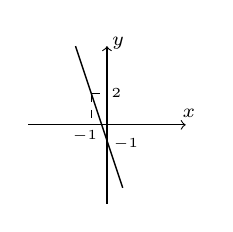
\begin{tikzpicture}[scale=0.2]
\tikzset {line01/.style={line width =0.5pt}}
\tikzset{line02/.style={line width =1pt}}
\tikzset{line03/.style={dashed,line width =0.5pt}}
%\filldraw [black] (0,0) circle (1pt);
\draw [->] (-5,0) -- (5,0);
\draw [->] (0,-5) -- (0,5);
\draw[line01] (-2,5) -- (1,-4);
\draw[line03] (-1,2) -- (-1,0);
\draw[line03] (-1,2) -- (0,2);
%\draw[line01] (0,-3) -- (-2,5);
\draw (0.6,2) node {\tiny $2$};
\draw (-1.4,-0.7) node {\tiny $-1$};
\draw (5.2,0.7) node {\scriptsize $x$};
\draw (1.2,-1.2) node {\tiny $-1$};
\draw (0.7,5.2) node {\scriptsize $y$};
\end{tikzpicture}$$
Значение $y=2$ достигается при $x=-1,$ а так как функция убывает, неравенство $y\leqslant2$ выполняется при $x\geqslant-1.$\\
